\documentclass[11pt, paper=a4]{scrartcl}

% CONFIG
\newcommand{\exptitle}{M\"o\ss bauer effect}       % long name of experiment 
\newcommand{\exptitleshort}{M\"o\ss bauer effect} % short name of experiment
\newcommand{\expdate}{04.04.2016}           % date of experiment
\newcommand{\exptutor}{Veronika Magerl}

% PACKAGES + MODIFICATIONS
%\usepackage[ngerman]{babel} %standard language stuff
\usepackage[T1]{fontenc}
\usepackage[utf8]{inputenc}
\usepackage{textgreek}

\usepackage{soul} %better underline
\setul{2pt}{.4pt} %set underline 2 pts below text and thickness to .4pt

\usepackage[fleqn]{amsmath}  % math
\usepackage{amssymb}

\usepackage{graphicx} %graphics
\usepackage{float} 

\usepackage[automark,headsepline]{scrlayer-scrpage} %headings
\pagestyle{scrheadings}
\ihead{\exptitleshort}
\ohead{\pagemark}
\cfoot{}

\usepackage{hyperref}
\hypersetup{
    unicode=true,          % non-Latin characters in Acrobat’s bookmarks
    pdftoolbar=true,       % show Acrobat’s toolbar?
    pdfmenubar=true,       % show Acrobat’s menu?
    pdffitwindow=false,    % window fit to page when opened
    pdfstartview={FitH},   % fits the width of the page to the window
    pdfnewwindow=true,     % links in new window
    colorlinks=true,       % false: boxed links; true: colored links
    linkcolor=blue,       % color of internal links (change box color with linkbordercolor)
    citecolor=green,       % color of links to bibliography
    filecolor=magenta,     % color of file links
    urlcolor=blue          % color of external links
}

\usepackage[labelfont=bf]{caption} % bold captions

\usepackage{chngcntr} % change behaviour of counters in different environments
\counterwithin{figure}{section}  % number figures per section
\numberwithin{equation}{section} % number equations per section
\numberwithin{table}{section}    % number tables per section

\usepackage{enumerate} % better way to config enumerates

\setcounter{tocdepth}{2} % table of contents depth

\setlength{\parindent}{0pt} % no indent on new paragraph

\usepackage{pdfpages} % include pdf files

\usepackage[nottoc,numbib]{tocbibind} % bibliography in TOC

\usepackage{isotope}
\usepackage{booktabs} %package for tables and settings
% NEW COMMANDS
\newcommand{\refeq}[1]{\overset{\text{\eqref{#1}}}{=}}

% DOCUMENT SETTINGS

\title{\exptitle}
\subtitle{}
\author{}
\date{\expdate}

% DOCUMENT
\begin{document}

\hypersetup{pageanchor=false} %stop page numbering (hyperref) to prevent for double page numers
\newcommand{\HRule}{\rule{\linewidth}{0.5mm}}
\begin{titlepage}
\begin{center}
  \textsc{\Large Fortgeschrittenen Praktikum II }\\[0.5cm]
  \HRule \\[0.4cm]
  { \huge \bfseries \exptitle}\\
  \HRule \\[0.5cm]
  \large \expdate\\[0.5cm]  
  Benjamin Winkelmann \\
  Peter Spalthoff \\
  \vspace{10pt}
  \large 
  Tutor: \exptutor \\[3cm]
  \vfill
  \normalsize
\end{center}
\end{titlepage}
\thispagestyle{empty}



\pagenumbering{Roman}
\setcounter{page}{1}


%\section*{Abstract}
In the experiment the absorption spectrum of stainless steel and natural iron are recored by using the Mössbauer effect. The Gamma radiation of a Fe-57 decay is Doppler shifted by moving the absorber relative to the source. This allows for a high relative resolution, enabling the measurement of the isometric shift in stainless steel $E_{iso}= \unit{8.61\pm0.24\cdot10^{-9}}{eV}$ and natural iron $\overline{E_{iso}} = \unit{(4.9\pm1.1)}{neV}$. Furthermore the Debye-Waller factor was calculated to be $f_s=0.51\pm0.08$.
\tableofcontents

\newpage
\listoffigures
\thispagestyle{empty}

\newpage
\hypersetup{pageanchor=false} %stop page numbering (hyperref) to prevent for double page numers

\clearpage
\pagenumbering{arabic}
\setcounter{page}{1}

%physical principles
\section{Goal of the experiment}
By measuring absorption of photons of the $14.4 kev$ transition of Fe-57, in stainless steel and natural iron, the isomeric shift, the effective absorber thickness, the  Debeye-Waller-factor of the source the lifetime of the excited Fe-57 state, the magnetic field at the location of the nucleus and the magnetic moment of the $14.4 ke$V state.

\section{physical principles}
\subsection{Interaction of Gamma radiation with matter}
Photons interact with matter in three major ways\cite{Demtröder}:
\paragraph{Photoelectric effect} \ \\
Shell electrons of atoms absorb photons and gain its energy, leaving the potential well of the atom and exiting the shell with the energy $E_e = E_\gamma-E_B$ with $E_B$ being the binding energy of the electron.
\paragraph{Compton scattering} \ \\
Compton Scattering is the elastic scattering of photons at quasi free  electrons ($E_B << E_\gamma$) and its wavelength $\lambda=2\pi c/\omega$ is shifted, depending on the scattering angle $\varphi$(see figure \ref*{eq:compton}):
\begin{equation}
\lambda_S -\lambda_0 = \frac{2 \pi \hbar}{m_e c}(1-cos(\varphi))
\label{eq:compton}
\end{equation}
\paragraph{Pair Production} \ \\
A photon can produce a positron electron pair if it has an energy of at least $2\cdot m_e=1.022MeV$ the photon is lost in the processes reducing the Intensity of the photon beam.\\ \ \\
Due to those processes the intensity of electromagnetic radiation decreases exponentially with penetration depth $d$:
\begin{equation}
I(d)=I_0 \cdot exp(-\mu d)
\end{equation}
where $\mu$ is the attenuation coefficient.
\begin{figure}[h]
	\centering
	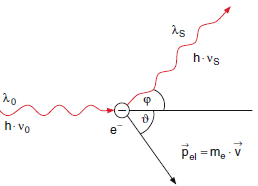
\includegraphics[width=0.5\linewidth]{graphics/Compton}
	\caption[Compton scattering]{Compton effect: A photon is scattered by a (quasi) free electron changing its direction by an angle $\varphi$\cite{Demtröder} }
	\label{fig:principles:Compton}
\end{figure}

\begin{figure}[H]
	\centering
	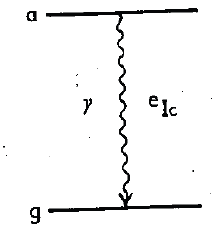
\includegraphics[height=0.18\textheight]{graphics/Emission}
	\caption[spontaneous $\gamma$ emission]{principle of spontaneous $\gamma$ emission of excited nuclei. Transitioning from an excited state ($E_a$) to the ground state ($E_g$) the nucleus emits a photon with energy $E_a-E_g=\hbar\dot \omega$ or transmits that energy directly to an electron of the atomic shell.\cite{Wegener}}
	\label{fig:principles:Emission}
\end{figure}
\subsection{Gamma Decay and resonance absorption}
Nuclei in excited states (energy $E_a$) can spontaneously transition into the ground (energy $E_g$) state. The energy $\Delta E$ the nucleus loses is either carried by an emitted photon (spontaneous emission) or directly gained by a shell electron (inner conversion). \\
In the case of spontaneous emission, the photon can be absorbed by a nucleus of the same kind which thereby transits into an excited state. This is called resonance absorption. However due to the recoil the nuclei receive this rarely happens for free atoms.
Consider the rest frame of a nucleus, that means its momentum is $p_0 = 0$. Now consider this nucleus decays by emitting a photon. Since the photon carries the momentum 
\begin{equation}
 p = \frac{E_\gamma}{c}= \frac{\hbar}{c}\cdot \omega
\label{eq:momentum}
\end{equation}
with the reduced Planck constant $\hbar$ and c the speed of light, and momentum is conserved the nucleus receives a recoil equal to the photons momentum and therefore also kinetic energy or recoil energy $R$. The emitted photon therefore has the energy \cite{Eyges}:
\begin{equation}
E_\gamma=\Delta E - \frac{p^2}{2m} = \Delta E - \frac{(\hbar \omega)^2}{2mc^2} =:\Delta E-R
\label{eq:recoil:emission}
\end{equation}
When the photon is absorbed the same applies: the absorbing nucleus receives the recoil $R$. This means for a photon to be absorbed, inducing a nuclear transition with $\Delta E$ the photon has to have the energy:
\begin{equation}
E_\gamma=\Delta E + R
\label{eq:recoil:absorbtion}
\end{equation}
In consequence the absorption spectrum is shifted relative to the emission spectrum (see fig \ref{fig:principles:lorentz} depending on the recoil energy $R$.

\begin{figure}[hpbt]
	\centering
	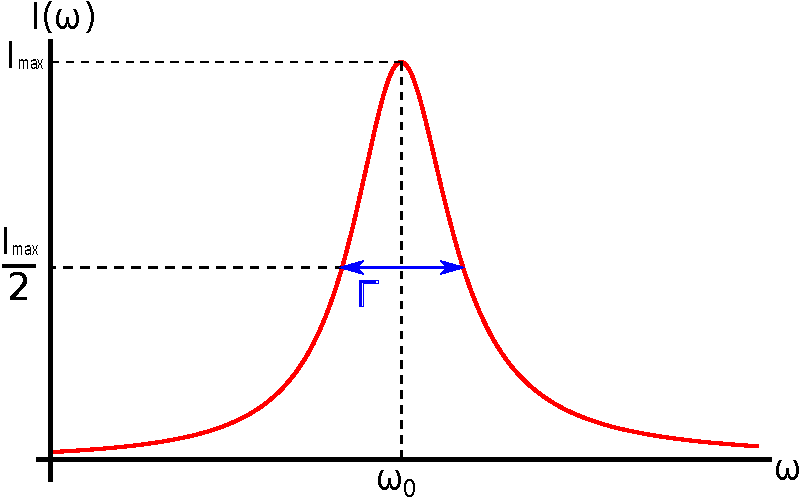
\includegraphics[height=0.25\textheight]{graphics/Lorentz.pdf}
	\caption[Lorentz distribution]{Lorentz distribution: $I(\omega) \propto \frac{1}{(\omega-\omega_0)^2+(\Gamma /2)^2}$\\}
	\label{fig:principles:lorentz}
\end{figure}

\subsection{Doppler shift}
Due to thermal motion the emitting nucleus and the absorbing nucleus have relative velocity $v$, shifting the frequency via Doppler effect:  
\begin{equation}
E_\gamma^{'} = E_\gamma (1+\frac{v}{c}) 
\label{eq:doppler shift}
\end{equation}
So the energy is changed by:
\begin{equation}
E_\gamma^{'} - E_\gamma = E_\gamma \frac{v}{c}
\label{eq:diffdopplershift}
\end{equation}


\subsection{Mößbauer effect}
The Mößbauer effect is the name for the phenomenon of \emph{recoilless emission} (or absorption). Revisiting equation \ref{eq:recoil:emission} one an see that the recoil energy $R=\frac{(\hbar \omega)^2}{2mc^2}$ is inversely proportional to the mass of the nucleus. In a solid it is possible for the whole lattice the absorb the recoil therefore increasing the recoiled mass enormously, so that $R\approx0$\footnote{this is a simplified description, for a more detailed one see \cite{Eyges} and \cite{Wegener} }. This effect means atoms that shows this behavior (In this experiment Fe-57) can emit photons, that can be reabsorbed by atoms of the same kind.

%\subsubsection{Einstein lattice}
%In the Einstein model the atoms of a lattice are described as three dimensional quantum mechanical oscillators, all with the same frequency $\omega_E$ This means the lattice can only increase its energy in quanta of $\hbar \omega_E$ so if $E_\gamma < \hbar \omega_E$ the absorption is recoilless.
%\subsubsection{Debye mdoel}
%In contrast to Einstein's model, this model allows for several frequencies, introducing a dispersion relation for the vibrational spectrum:
%\begin{equation}
%\omega = c_S\cdot k
%\end{equation}
%Where $c_S$ is the speed of the sound and k is the wave vector 
\subsection{Debye-Waller factor}
The Debye-Waller factor is the ratio of recoilless absorption.
\begin{equation}
f = exp \left[ -\frac{3R}{2k \cdot \Theta_D} \left(1+ \frac{4T^2}{\Theta_D^2}\int_{0}^{\Theta/T}\frac{xdx}{e^x-1}\right) \right]
\end{equation}
Where $R$ is the recoil energy, $k$ the Boltzmann constant, $\Theta_D$ the Debye temperature. 
If the temperature is low $T<<\Theta_D$ this can be simplified to:
\begin{equation}
f \approx exp\left[ -\frac{3R}{k \cdot \Theta_D} \left( \frac{3}{2}+\frac{\pi^2 T^2}{\Theta_D^2}\right) \right]
\end{equation}

\begin{figure}
\centering
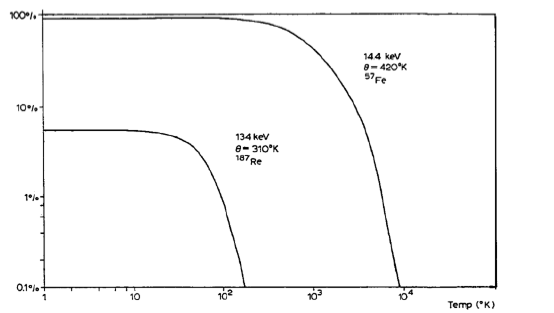
\includegraphics[width=0.7\linewidth]{graphics/Debeyfactor}
\caption[Debey factors]{Debye factor as a function of temperature in Fe-57 and Re-187. At room temperature Fe-57 has a ratio of recoilless emission absorption of 0.91}
\label{fig:principles:Debeyfactor}
\end{figure}

\subsection{Isomer shift}
Since electrons of an atomic shell are kept within the coulomb potential of the nucleus their potential energy depends on the charge distribution in the nucleus. Transitioning to an excited state affects this distribution therefore also affecting the potential energy of the electrons. This change in energy shifts the frequency that an absorbed photon must have to induce the transition\cite{Wegener}.
\subsection{Hyperfine splitting}
The nucleus has magnetic moment ($\mu_I$) and spin $I$. In a surrounding magnetic field $H$ the energy level splits into $2I+1$ sub-energy levels. The sub-sates are characterized by the magnetic quantum number $m_I = -I,I+1..,I-1,I$ and the energy difference induced is:
\begin{equation}
E_{HFS}=\frac{\mu_I m_I H}{I}
\end{equation}
\begin{figure}[H]
\centering
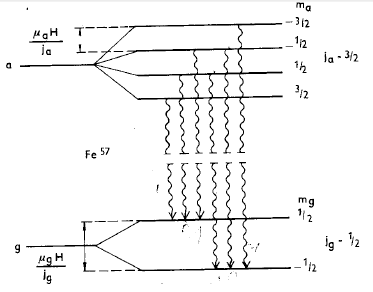
\includegraphics[width=0.5\linewidth]{graphics/HFS}
\caption[Hyperfine splitting Fe-57]{Hyperfine splitting for Fe-57 in magnetic field H for the ground state g ($I_g = 1/2$) and the excited state ($I_a=3/2$).\cite{Wegener}}
\label{fig:HFS}
\end{figure}
The transition $m_a \rightarrow m_g$ emits photons with energy $\omega$:
\begin{equation}
E_\gamma(m_a,m_g) = E_0 - \left( \frac{\mu_a m_a}{I_a}-\frac{\mu_g m_g}{I_g}\right) H
\label{eq:HFS}
\end{equation}




\section{Experimental setup}
\subsection{Method}
To measure the absorption spectra of stainless steel and natural iron, we irradiate the samples with the $14.4keV$ $\gamma$-radiation emitted by a radioactive source. To vary the frequency a motor is used to move the absorber relative to the source (Doppler shift see  \ref{eq:diffdopplershift}). By repeating this measurement for different absorber velocities a spectrum is recorded.\\
\subsection{Setup}
\begin{figure}[hbt]
\centering
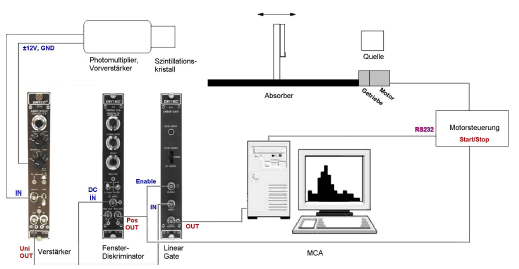
\includegraphics[width=1.0\linewidth]{graphics/Aufbau}
\caption[Setup overview ]{Overview of the experimental setup}
\label{fig:Aufbau}
\end{figure}

The setup consists of the $\gamma$ source, the absorber on a track, the motor used to move the absorber at constant speeds relative to the source and as the photon detector a scintillator is used. The light signal of the scintillator turned into an electric signal by a photomultiplier. This signal is amplified and shaped in the amplifier. The amplifier has two exits, one of which is connected to a single channel analyzer (SCA). If the signal pulse is within an adjustable window the SCA sends a standardized signal and enables the linear gate, which is also connected to the amplifier via a delay to ensure simultaneity of the signals. If the linear gate is enabled when it receives a signal from the amplifier it transmits the amplifier signal to the multichannel analyzer (MCA), which is read out with a Computer. The second output of the SCA is connected to a counter, which also can be read out with the Computer.

\subsection{The source Co-57}
\isotope[57]{Co} decays via electron capture with a branching ratio of $99.8 \%$ and a half life of 270d into an iron in an excited state $\isotope[57]{Fe^*}$. This state decays with a half life of 9ns an branching ratio of $88\%$ into the $14.4keV$ excited state which finally decays to the ground state (Branching ratio for $\gamma-decay$ is $10\%$) \ref{fig:principles:Zerfallsschema2}. 
\begin{figure}[hbt]
	\centering
	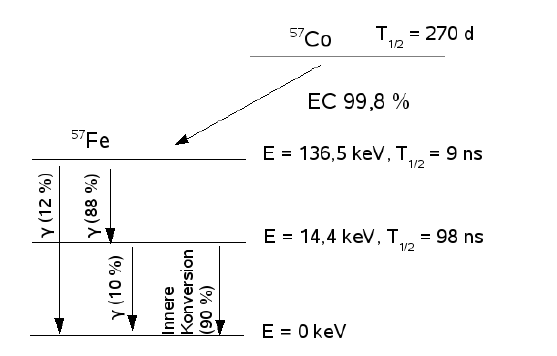
\includegraphics[width=0.5\linewidth]{graphics/Zerfallsschema2}
	\caption[Co-57 decay]{decay series of Cobalt-57}
	\label{fig:principles:Zerfallsschema2}
\end{figure}
\subsection{Procedure}
\subsubsection{MCA calibration}
To calibrate the MCA the spectra of Cu, Rb, Mo, Ag, Ba, and Tb are measured for 300s each. For the Cu no peak
\subsubsection{background measurement}

\newpage
\begin{thebibliography}{9}
\bibitem{Wegener}
Wegener, Horst. "Der Mößbauer Effekt und seine Anwendungen". Mannheim 1966
\bibitem{Demtröder}
Demtröder, Wolfgang. Experimentalphysik 3 Atome, Moleküle und Festkörper
\bibitem{Codata}
P.J.Mohr, D.B.Newell, and B.N. Taylor:\\ "CODATA Recommended Values of the Fundamental Physical Constants: 2014". http://physics.nist.gov/cuu/Constants/index.html(26.04.2016)
\bibitem{jakobs}
Jakobs, Karl. Experimentelle Methoden der Teilchenphysik. Vorlesungsskript 2014
\bibitem{Eyges}
Eyges, Leonard. Physics of the Mössbauer effect. 1965
\bibitem{anleitung}
A.Zwerger(2007), S.Winkelmann(1/2011), M.Köhli (2/2011). Versuchsanleitung Fortgeschrittenen Praktikum Teil II - Der Mößbauer-Effekt. 2012
\bibitem{khwz}
M.Köhler(8/2010), M.köhli (4/2011). Versuchanleitung Fortgeschrittenen Praktikum Teil I - Kurze Halbwertszeiten
\end{thebibliography}



\end{document}
